\chapter{Криптографические протоколы}\index{протокол!криптографический}\label{chapter-protocols}
\selectlanguage{russian}

\section{Основные понятия}

Для успешного выполнения любых целей по защите информации необходимо участие в процессе защиты нескольких субъектов, которые по определённым правилам будут выполнять технические или организационные действия, криптографические операции, взаимодействовать друг с другом, например, передавая сообщения или проверяя личности друг друга.

Формализация подобных действий делается через описание протокола. \emph{Протокол} -- описание распределённого алгоритма, в процессе выполнения которого два или более участников последовательно выполняют определённые действия и обмениваются сообщениями\footnote{Здесь и далее в этом разделе определения даны на основе~\cite{Cheremushkin:2009}.}.

Под участником\index{участник!протокола} (субъектом\index{субъект!протокола}, стороной\index{сторона!протокола}) протокола понимают не только людей, но и приложения, группы людей или целые организации. Формально участниками считают только тех, кто выполняет активную роль в рамках протокола. Хотя при создании и описании протоколов забывать про пассивные стороны тоже не стоит. Например, пассивный криптоаналитик\index{криптоаналитик!пассивный} формально не является участником протоколов, но многие протоколы разрабатываются с учётом защиты от таких <<неучастников>>.

Протокол состоит из \emph{циклов}\index{цикл!протокола} (\langen{round}) или \emph{проходов}\index{проход!протокола} (\langen{pass}). Цикл -- временной интервал активности только одного участника. За исключением самого первого цикла протокола, обычно начинается приёмом сообщения, а заканчивается -- отправкой.

Цикл (или проход) состоит из \emph{шагов} (действий, \langen{step, action}) -- конкретных законченных действий, выполняемых участником протокола. Например:
\begin{itemize}
	\item генерация нового (случайного) значения;
	\item вычисление значений функции;
	\item проверка сертификатов, ключей, подписей, и др.;
	\item приём и отправка сообщений.
\end{itemize}

Прошедшая в прошлом или даже просто теоретически описанная реализация протокола для конкретных участников называется \emph{сеансом}\index{сеанс!протокола}. Каждый участник в рамках сеанса выполняет одну или несколько \emph{ролей}. В другом сеансе протокола участники могут поменяться ролями и выполнять уже совсем другие функции.

Можно сказать, что протокол прескрептивно описывает правила поведения каждой роли в протоколе. А сеанс это дескриптивное описание (возможно теоретически) состоявшейся в прошлом реализации протокола.

Пример описания протокола.
\begin{enumerate}
	\item Участник с ролью <<Отправитель>> должен отправить участнику с ролью <<Получатель>> сообщение.
	\item Участник с ролью <<Получатель>> должен принять от участника с ролью <<Отправитель>> сообщение.
\end{enumerate}

Пример описания сеанса протокола.
\begin{enumerate}
	\item 1-го апреля в 13:00 Алиса отправила Бобу сообщение.
	\item 1-го апреля в 13:05 Боб принял от Алисы сообщение.
\end{enumerate}

\emph{Защищённым протоколом}\index{протокол!защищённый} или \emph{протоколом обеспечения безопасности}\index{протокол!обеспечения безопасности} будет называть протокол, обеспечивающий выполнение хотя бы одной защитной функции~\cite{ISO:7498-2:1989}:
\begin{itemize}
	\item аутентификация сторон и источника данных,
	\item разграничение доступа,
	\item конфиденциальность,
	\item целостность,
	\item невозможность отказа от факта отправки или получения.
\end{itemize}

Если защищённый протокол предназначен для выполнения функций безопасности криптографической системы, или если в процессе его исполнения используются криптографические алгоритмы, то такой протокол будем называть \emph{криптографическим}\index{протокол!криптографический}.

\section{Запись протоколов}
Для записи протоколов, связанных с реализацией функций защиты информации, не используют выражения вроде <<участник с ролью <<Отправитель>>>>, а заменяют их на краткие обозначения вроде <<отправитель>> или используют общепринятые экземплификанты\footnote{\emph{Экземплификант} или \emph{экземплификатив} -- конкретное понятие или имя собственное, используемое в качестве примера для обозначения неизвестного места или личности. (Википедия, свободная энциклопедия; 5 июля 2019)}: Алиса, Боб, Клара, Ева и~т.\,д. При этом используют следующие соглашения.

\begin{itemize}
	\item Алиса, Боб (от \langen{A, B}) -- отправитель и получатель.
	\item Карл, Клара, Чарли (от \langen{C}) -- равноправная третья сторона.
	\item Ева (от \langen{eavesdropper}) -- пассивный криптоаналитик.
	\item Меллори (от \langen{malicious}) -- активный криптоаналитик.
	\item Трент (от \langen{trust}) -- доверенная сторона.
\end{itemize}

Не существует общепринятого формата записи протоколов, они могут отличаться как по внешнему виду, так и по полноте описания. Например, вот наиболее полный формат записи протокола Диффи~---~Хеллмана\index{протокол!Диффи~---~Хеллмана}.

\begin{itemize}
	\item Предварительный этап.
	\begin{itemize}
		\item Все стороны выбрали общие $g$ и $p$.
	\end{itemize}
	\item Проход 1.
	\begin{itemize}
		\item Алиса генерирует случайное $a$.
		\item Алиса вычисляет $A = g^a \bmod p$.
		\item Алиса отправляет Бобу $A$.
	\end{itemize}
	\item Проход 2.
	\begin{itemize}
		\item Боб принимает от Алисы $A$.
		\item Боб генерирует случайное $b$.
		\item Боб вычисляет $B = g^b \bmod p$.
		\item Боб отправляет Алисе $B$.
		\item Боб вычисляет $s = A^b \bmod p$.
	\end{itemize}
	\item Проход 2.
	\begin{itemize}
		\item Алиса принимает от Боба $B$.
		\item Алиса вычисляет $s = B^a \bmod p$.
	\end{itemize}
	\item Результат протокола.
	\begin{itemize}
		\item Стороны вычислили общий сеансовый ключ $s$.
	\end{itemize}
\end{itemize}

Теперь сравните с краткой записью того же самого протокола.
\begin{enumerate}
	\item $A \to B : A = g^a \bmod p$
	\item $B \to A : B = g^b \bmod p$
\end{enumerate}

В краткой записи опускаются инициализация и предварительные требования, вычисления непередаваемых данных (в данном примере -- общего сеансового ключа $s$), а также любые проверки.

В данном пособии мы будем придерживаться промежуточного формата записи.

\begin{enumerate}
	\item[(1)] Алиса генерирует $a$.
	\item[] $Alice \to \left\{ A = g^a \bmod p \right\} \to Bob$.
	\item[(2)] Боб генерирует $b$.
	\item[] Боб вычисляет $s = A^b \bmod p$.
	\item[] $Bob \to \left\{ B = g^b \mod p \right\} \to Bob$.
	\item[(3)] Алиса вычисляет $s = B^a \bmod p$.
\end{enumerate}

Также условимся о правилах записи случая, когда активный криптоаналитик (Меллори) выдаёт себя за легального пользователя.

\[
\begin{array}{llllc}
(1) & A                & \to M \left(B\right) & : & A   = g^a     \bmod p, \\ 
(2) & M \left(A\right) & \to B                & : & A^* = g^{a^*} \bmod p, \\ 
(3) & B                & \to M \left(A\right) & : & B   = g^b     \bmod p, \\ 
(4) & M \left(B\right) & \to A                & : & B^* = g^{b^*} \bmod p. \\
\end{array}
\]

Либо, отводя отдельный столбец для каждого участника.
\[
\begin{array}{lllclllc}
	(1) & A  & \to   & M \left(B\right) & {}    & {} & : & A = g^a     \bmod p, \\ 
	(2) & {} & {}    & M \left(A\right) & \to   & B  & : & A^* = g^{a^*} \bmod p, \\ 
	(3) & {} & {}    & M \left(A\right) & \gets & B  & : & B   = g^b     \bmod p, \\ 
	(4) & A  & \gets & M \left(B\right) & {}    & {} & : & B^* = g^{b^*} \bmod p. \\
\end{array}
\]

Для сокращения описания и упрощения сравнения разных протоколов используют следующие соглашения об обозначениях передаваемых данных.

\begin{itemize}
	\item $M$ (от \langen{message}) -- сообщение в исходном виде, открытый текст вне зависимости от кодировки. То есть под $M$ может пониматься и исходный текст в виде текста или, например, звука, либо уже некоторое число или массив бит, однозначно соответствующие этому сообщению.
	\item $K$ (от \langen{key}) -- некоторый ключ. Без дополнительных уточнений обычно обозначает секретный сеансовый ключ.
	\item $K_A$ -- общий секретный ключ между Алисой и Трентом (для симметричных криптосистем).
	\item $K_A$ -- открытый ключ Алисы (для асимметричных криптосистем).
	\item $E_K \left( \dots \right)$ (от \langen{encrypt}) -- данные, зашифрованные на ключе $K$.
	\item $S_K \left( \dots \right)$ (от \langen{sign}) -- данные \emph{и} соответствующая цифровая подпись на открытом ключе $K$.
	\item $T_A$, $T_B$ (от \langen{timestamp}) -- метки времени от соответствующих участников.
	\item $R_A$, $R_B$ (от \langen{random}) -- случайные числа, выбранные соответствующими участниками.
\end{itemize}

\input{protocols-properties}

\section{Протоколы распространения ключей}

Задача распространения ключей является одной из множества задач построения надёжной сети общения многих абонентов. Задача состоит в получении в нужный момент времени двумя легальными абонентами сети секретного сессионного ключа шифрования (и аутентификации сообщений). Хорошим решением данной задачи будем считать такой протокол распространения ключей, который удовлетворяет следующим условиям.

\begin{itemize}
	\item В результате работы протокола между двумя абонентами должен быть сформирован секретный сессионный ключ.
	\item Успешное окончание работы протокола распространения ключей должно означать успешную взаимную аутентификацию абонентов. Не должно быть такого, что протокол успешно завершился с точки зрения одной из сторон, а вторая сторона при этом представлена злоумышленником.
	\item К участию в работе протокола должны допускаться только легальные пользователи сети. Внешний пользователь не должен иметь возможность получить общий сессионный ключ с кем-либо из абонентов.
	\item Добавление нового абонента в сеть (или исключение из неё) не должно требовать уведомления всех участников сети.
\end{itemize}

Последнее требование сразу исключает такие варианты протоколов, в которых каждый из абонентов знал бы некоторый мастер-ключ общения с любым другим участником. Данные варианты плохи тем, что с ростом системы количество пар мастер-ключей <<абонент-абонент>> растёт как квадрат от количества участников. Поэтому большая часть рассматриваемых решений состоит в том, что в сети выделяется один или несколько доверенных центров T (\langen{Trent}, от \langen{trust}), которые как раз и владеют информацией обо всех легальных участниках сети и их ключах. Они же будут явно или неявно выступать одним из участников протоколов по формированию сеансовых ключей.

\begin{figure}[!htb]
    \centering
    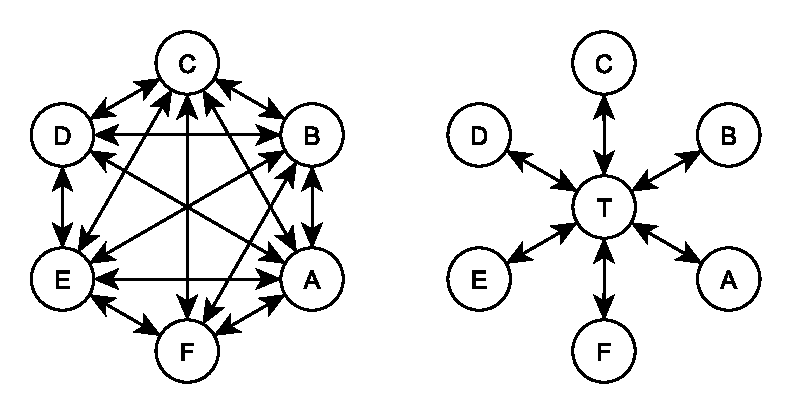
\includegraphics[width=0.8\textwidth]{pic/key_distribution-networks}
    \caption{Варианты сетей без выделенного доверенного центра и с выделенным доверенным центром T\label{fig:key_distribution-networks}}
\end{figure}

Важным моментом при анализе решений данной задачи является то, что сессионные ключи, вырабатываемые в конкретный момент времени, являются менее надёжными, чем мастер-ключи, используемые для генерации сессионных. В частности, нужно предполагать, что хотя злоумышленник не может получить сессионный ключ во время общения абонентов, он может сделать это по прошествии некоторого времени (дни, недели, месяцы). И хотя знание этого сессионного ключа поможет злоумышленнику расшифровать старые сообщения, он не должен иметь возможность организовать новую сессию с использованием уже известного ему сессионного ключа.

\section{Симметричные протоколы}
\selectlanguage{russian}

Как отмечено ранее в разделе~\ref{section-protocols-classification} про классификацию протоколов, к симметричным будем относить те протоколы, которые используют примитивы только классической криптографии на секретных ключах. К ним относятся уже известные блочные шифры, криптографически стойкие генераторы псевдослучайных чисел (КСГПСЧ) и хэш-функции.

\input{protocols-wide-mouth_frog}

\input{protocols-needham-schroeder}

\input{protocols-kerberos}


\input{protocols-three-pass}

\input{protocols-asymmetric}

\input{protocols-quantum}
